% Options for packages loaded elsewhere
\PassOptionsToPackage{unicode}{hyperref}
\PassOptionsToPackage{hyphens}{url}
%
\documentclass[
]{article}
\usepackage{amsmath,amssymb}
\usepackage{iftex}
\ifPDFTeX
  \usepackage[T1]{fontenc}
  \usepackage[utf8]{inputenc}
  \usepackage{textcomp} % provide euro and other symbols
\else % if luatex or xetex
  \usepackage{unicode-math} % this also loads fontspec
  \defaultfontfeatures{Scale=MatchLowercase}
  \defaultfontfeatures[\rmfamily]{Ligatures=TeX,Scale=1}
\fi
\usepackage{lmodern}
\ifPDFTeX\else
  % xetex/luatex font selection
\fi
% Use upquote if available, for straight quotes in verbatim environments
\IfFileExists{upquote.sty}{\usepackage{upquote}}{}
\IfFileExists{microtype.sty}{% use microtype if available
  \usepackage[]{microtype}
  \UseMicrotypeSet[protrusion]{basicmath} % disable protrusion for tt fonts
}{}
\makeatletter
\@ifundefined{KOMAClassName}{% if non-KOMA class
  \IfFileExists{parskip.sty}{%
    \usepackage{parskip}
  }{% else
    \setlength{\parindent}{0pt}
    \setlength{\parskip}{6pt plus 2pt minus 1pt}}
}{% if KOMA class
  \KOMAoptions{parskip=half}}
\makeatother
\usepackage{xcolor}
\usepackage[margin=1in]{geometry}
\usepackage{graphicx}
\makeatletter
\def\maxwidth{\ifdim\Gin@nat@width>\linewidth\linewidth\else\Gin@nat@width\fi}
\def\maxheight{\ifdim\Gin@nat@height>\textheight\textheight\else\Gin@nat@height\fi}
\makeatother
% Scale images if necessary, so that they will not overflow the page
% margins by default, and it is still possible to overwrite the defaults
% using explicit options in \includegraphics[width, height, ...]{}
\setkeys{Gin}{width=\maxwidth,height=\maxheight,keepaspectratio}
% Set default figure placement to htbp
\makeatletter
\def\fps@figure{htbp}
\makeatother
\setlength{\emergencystretch}{3em} % prevent overfull lines
\providecommand{\tightlist}{%
  \setlength{\itemsep}{0pt}\setlength{\parskip}{0pt}}
\setcounter{secnumdepth}{-\maxdimen} % remove section numbering
\usepackage{booktabs}
\usepackage{longtable}
\usepackage{array}
\usepackage{multirow}
\usepackage{wrapfig}
\usepackage{float}
\usepackage{colortbl}
\usepackage{pdflscape}
\usepackage{tabu}
\usepackage{threeparttable}
\usepackage{threeparttablex}
\usepackage[normalem]{ulem}
\usepackage{makecell}
\usepackage{xcolor}
\ifLuaTeX
  \usepackage{selnolig}  % disable illegal ligatures
\fi
\IfFileExists{bookmark.sty}{\usepackage{bookmark}}{\usepackage{hyperref}}
\IfFileExists{xurl.sty}{\usepackage{xurl}}{} % add URL line breaks if available
\urlstyle{same}
\hypersetup{
  pdftitle={2024-07-04 skeeter forecast},
  hidelinks,
  pdfcreator={LaTeX via pandoc}}

\title{2024-07-04 skeeter forecast}
\author{}
\date{\vspace{-2.5em}}

\begin{document}
\maketitle

Good afternoon! Here is your Skeeter report for July 04, 2024.

~

Today we counted 18 skeeter rafts. The closest prediction today was made
by Z with a prediction of 14. Get your predictions in before tomorrow's
count for a chance to show off your prediction skills!

\begin{figure}

{\centering 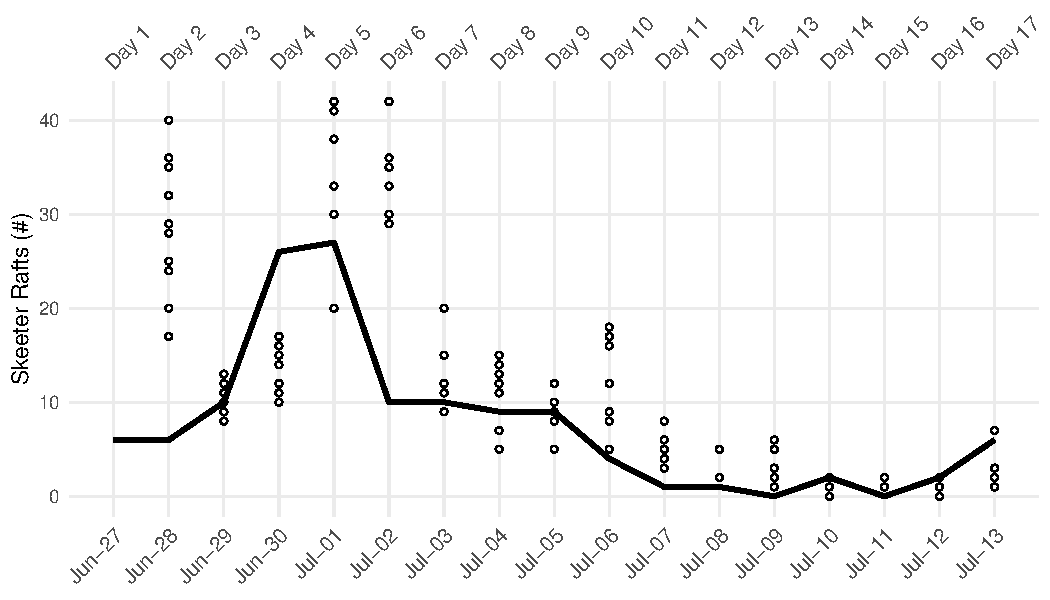
\includegraphics{skeeter-forecast-template_files/figure-latex/time series-1} 

}

\caption{Daily predictions (past = grey circles, current = black circles) and observations (black line) of mosquito rafts counted in mesocosms.}\label{fig:time series}
\end{figure}

To measure prediction accuracy, we will calculate the mean absolute
error,

\[MAE = \frac{\sum_{i}^{n}|y_{i} - x_{i}|}{n}\]

where, \(y_i\) is the prediction, \(x_i\) is the observed value, and
\(n\) is the number of observations.

\newpage

\subsubsection{Rankings}\label{rankings}

\begin{longtable}[t]{lrrrrrrrrr}
\caption{\label{tab:rankings table}The rankings to date are:}\\
\toprule
name & 2024-06-28 & 2024-07-02 & 2024-07-03 & 2024-07-04 & 2024-06-29 & 2024-06-27 & 2024-06-30 & 2024-07-01 & MAE\\
\midrule
GD & 8 & 16 & -5 & -5 & NA & NA & NA & NA & 8.50000\\
JMR & 20 & NA & -9 & -11 & -9 & NA & NA & NA & 12.25000\\
CRG & 13 & NA & NA & NA & NA & NA & NA & NA & 13.00000\\
Observed & -6 & -10 & -10 & -9 & -10 & -6 & -26 & -27 & 13.00000\\
JRJ & 16 & 22 & 0 & -6 & -10 & NA & -35 & -12 & 14.42857\\
\addlinespace
ZC & 5 & 15 & -8 & -4 & -7 & NA & -40 & -24 & 14.71429\\
EAC & 17 & 13 & -8 & -10 & NA & NA & -38 & -13 & 16.50000\\
JRB & 23 & 10 & -11 & -13 & -8 & NA & -36 & -21 & 17.42857\\
ARM & 12 & 10 & -9 & -7 & NA & NA & -42 & -34 & 19.00000\\
AM & 24 & 9 & NA & NA & -12 & NA & -41 & -16 & 20.40000\\
\addlinespace
JD & 28 & NA & NA & -11 & -11 & NA & -37 & -24 & 22.20000\\
\bottomrule
\end{longtable}

\subsubsection{Cumulative patterns}\label{cumulative-patterns}

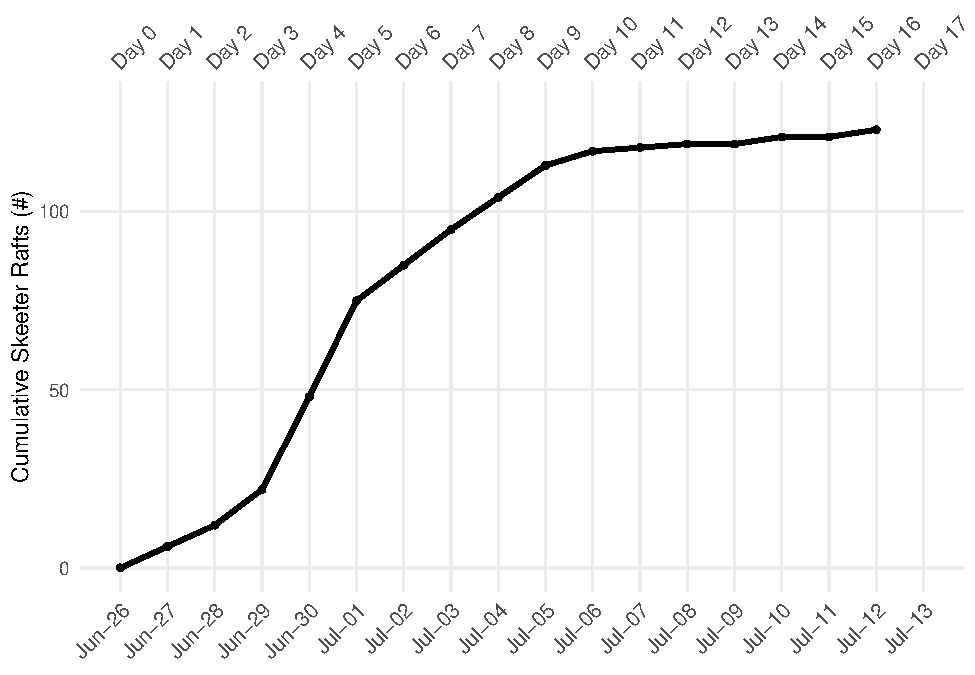
\includegraphics{skeeter-forecast-template_files/figure-latex/cumulative patterns-1.pdf}

\subsection{Forecasts}\label{forecasts}

Here are a few different models to forecast raft counts for 2024-07-05.

\subsubsection{Previous value}\label{previous-value}

The simplest prediction is to simply predict the previous raft count.

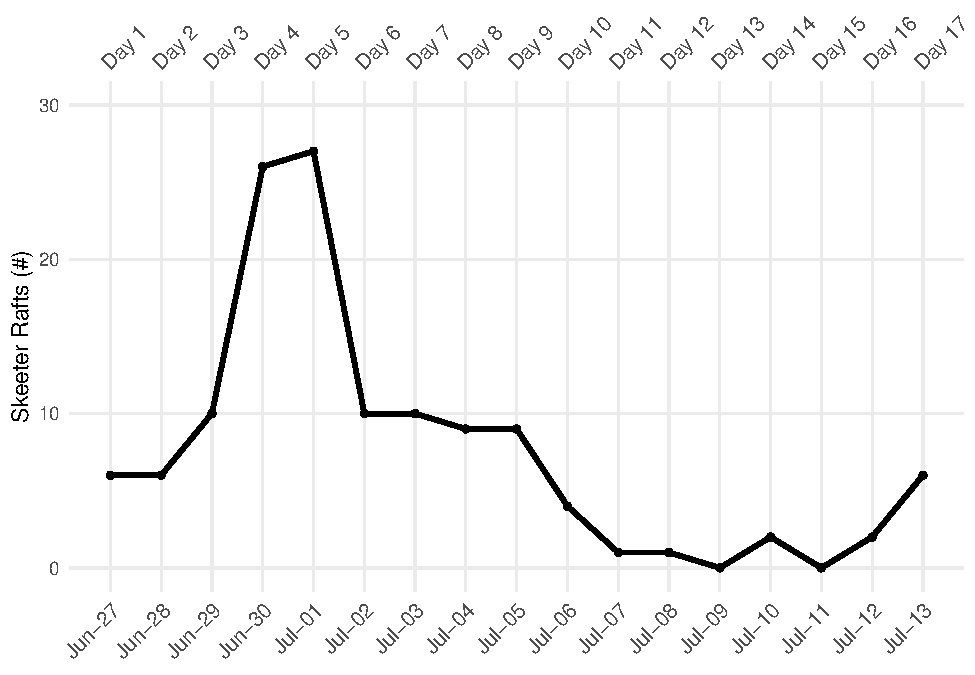
\includegraphics{skeeter-forecast-template_files/figure-latex/last value-1.pdf}

\begin{longtable}[t]{rrrrr}
\caption{\label{tab:last value accuracy}Mean predictive deviation of last value approach}\\
\toprule
2024-06-28 & 2024-06-29 & 2024-06-30 & 2024-07-01 & MAE\\
\midrule
-6 & -14 & -42 & -28 & 22.5\\
\bottomrule
\end{longtable}

\subsubsection{Global Average}\label{global-average}

Another simple prediction is to use the global average. This method
allows for a calculation of uncertainty based on the variation we
observe over time. Importantly, day-to-day variability in egg raft
numbers is not related to any process, but arises from random noise
centered around some relatively fixed mean value.

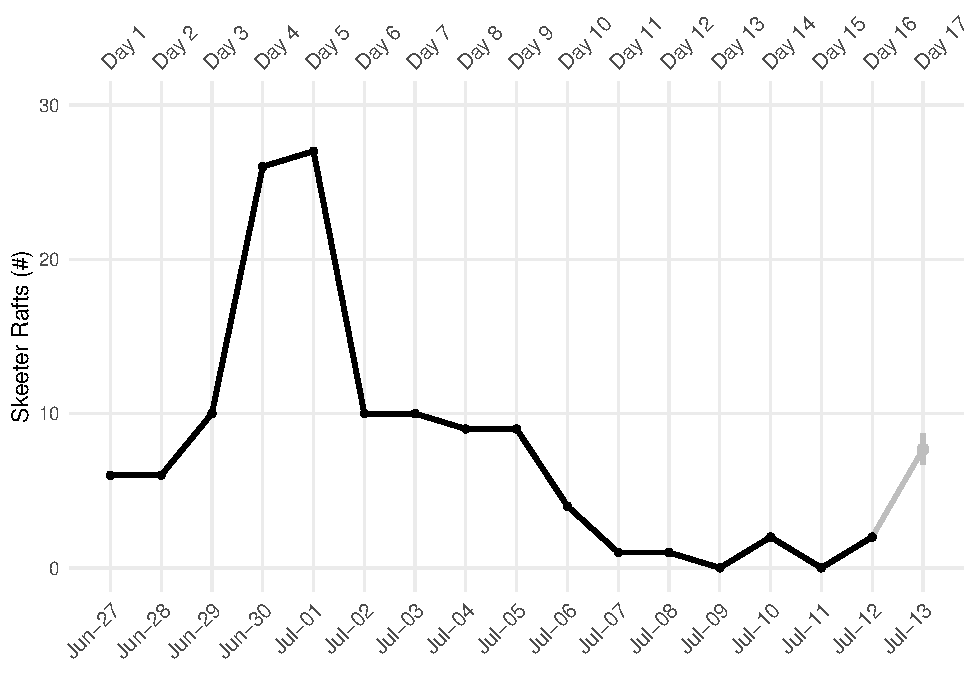
\includegraphics{skeeter-forecast-template_files/figure-latex/global average-1.pdf}

\begin{longtable}[t]{rrrrr}
\caption{\label{tab:global average accuracy}Mean predictive deviation of global average approach}\\
\toprule
2024-06-28 & 2024-06-29 & 2024-06-30 & 2024-07-01 & MAE\\
\midrule
-6 & -14 & -44.66667 & -42 & 26.66667\\
\bottomrule
\end{longtable}

However, this approach ignores an important bit of information---the
fact that egg rafts are counts and can only take whole numbers (i.e.,
1,2,3,\ldots).

\subsection{More complex predictions}\label{more-complex-predictions}

We can start to make more complex predictions. The best way to begin
this is to switch to making predictions at the mesocosm-level and scale
up to total counts. This will allow us to possibly include more specific
information to the experiment. As the global average example above
highlighted, we have to think about the type of data we are taking, in
this case counts. There are a number of distributions available for use
with count data such as the Poisson and Negative Binomial distributions.
Let's take a look at these distributions compared to the most recent
distribution of counts.

\begin{figure}
\centering
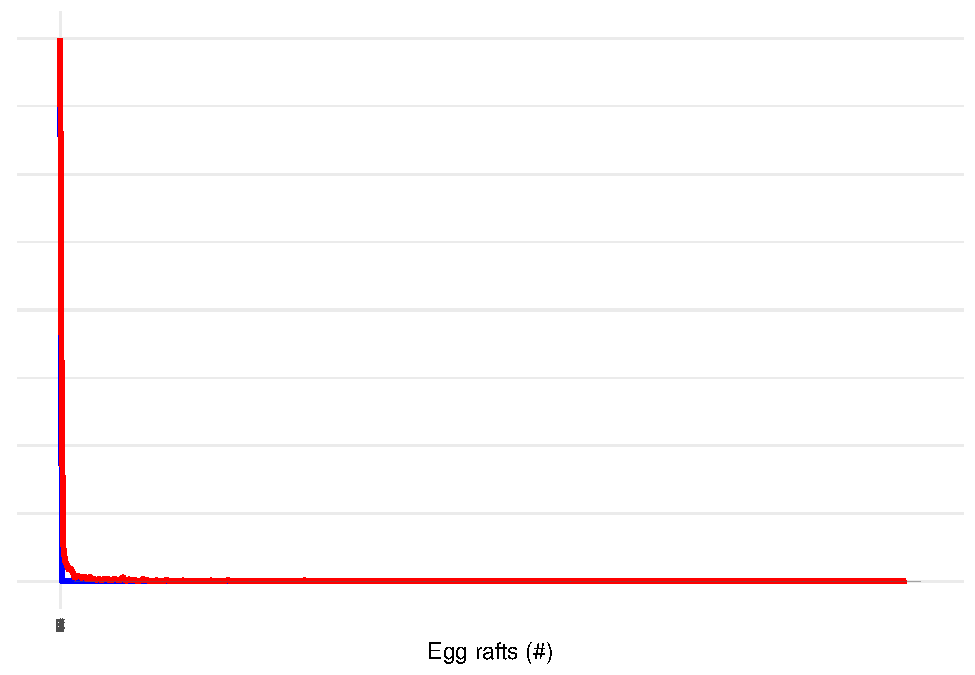
\includegraphics{skeeter-forecast-template_files/figure-latex/meso count hist-1.pdf}
\caption{The distribution of egg raft counts from the most recent
sampling (bars). We can see the difference in the predictions from the
Poisson (blue line) and Negative Binomial (red line) distributions
compared to the Guassian (black lines).}
\end{figure}

\subsubsection{Poisson}\label{poisson}

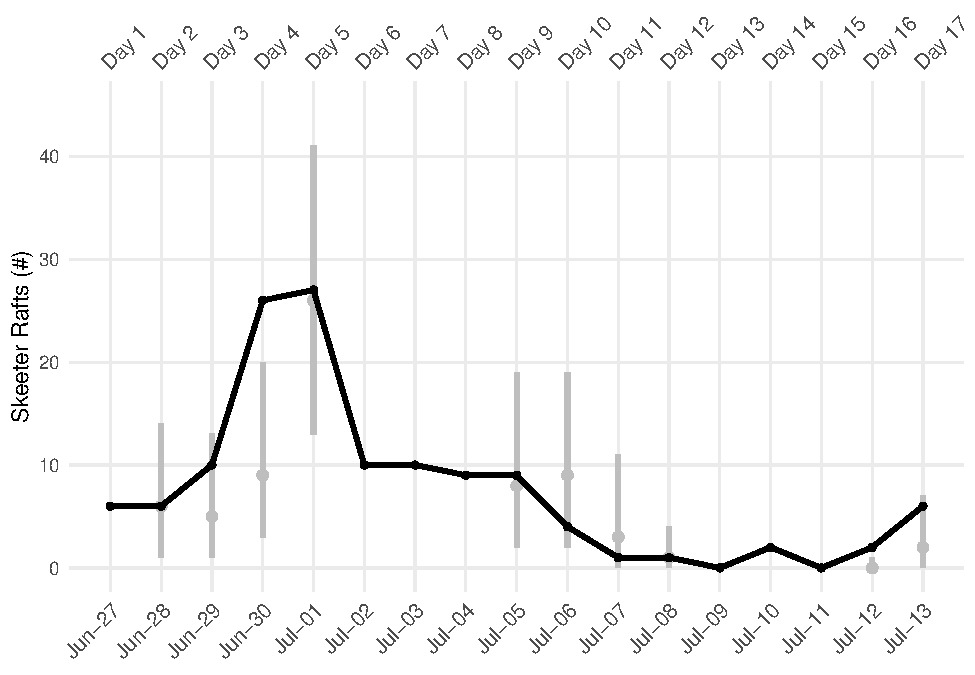
\includegraphics{skeeter-forecast-template_files/figure-latex/pois simple plot-1.pdf}

\begin{longtable}[t]{rrrrr}
\caption{\label{tab:pois simple accuracy}Mean predictive error of a simple Poisson model}\\
\toprule
2024-06-28 & 2024-06-29 & 2024-06-30 & 2024-07-01 & MAE\\
\midrule
-6 & -15 & -43 & -28 & 23\\
\bottomrule
\end{longtable}

\subsubsection{Negative Binomial}\label{negative-binomial}

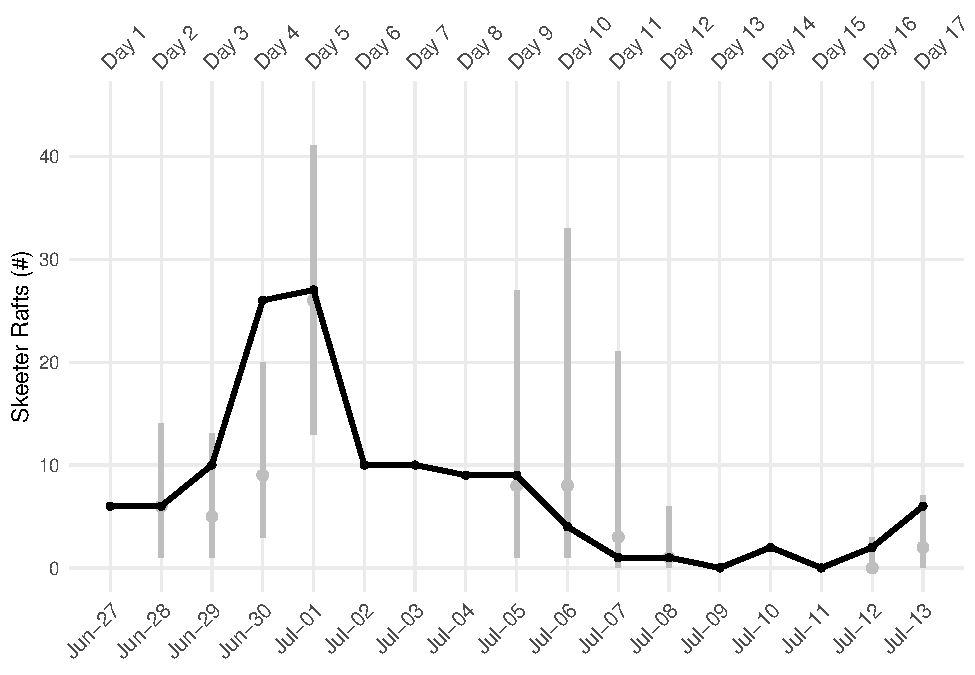
\includegraphics{skeeter-forecast-template_files/figure-latex/nb simple plot-1.pdf}

\begin{longtable}[t]{rrrrr}
\caption{\label{tab:nb simple accuracy}Mean predictive error of a simple Negative Binomial model}\\
\toprule
2024-06-28 & 2024-06-29 & 2024-06-30 & 2024-07-01 & MAE\\
\midrule
-6 & -15 & -43 & -28 & 23\\
\bottomrule
\end{longtable}

\subsection{Using our experimental design for prediction of MBs skeeter
rafts}\label{using-our-experimental-design-for-prediction-of-mbs-skeeter-rafts}

\subsubsection{Poisson}\label{poisson-1}

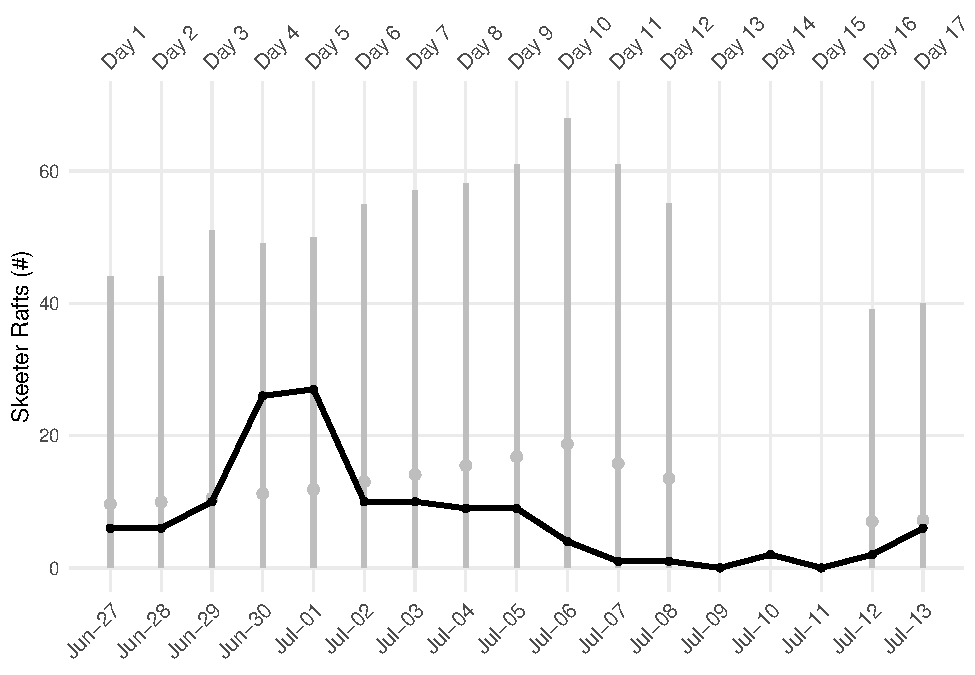
\includegraphics{skeeter-forecast-template_files/figure-latex/pois glmm plot-1.pdf}

\begin{longtable}[t]{rrrrr}
\caption{\label{tab:pois glmm accuracy}Mean predictive error of a simple Poisson model}\\
\toprule
2024-06-28 & 2024-06-29 & 2024-06-30 & 2024-07-01 & MAE\\
\midrule
-6 & -15 & -43 & -28 & 23\\
\bottomrule
\end{longtable}

\subsubsection{Negative Binomial}\label{negative-binomial-1}

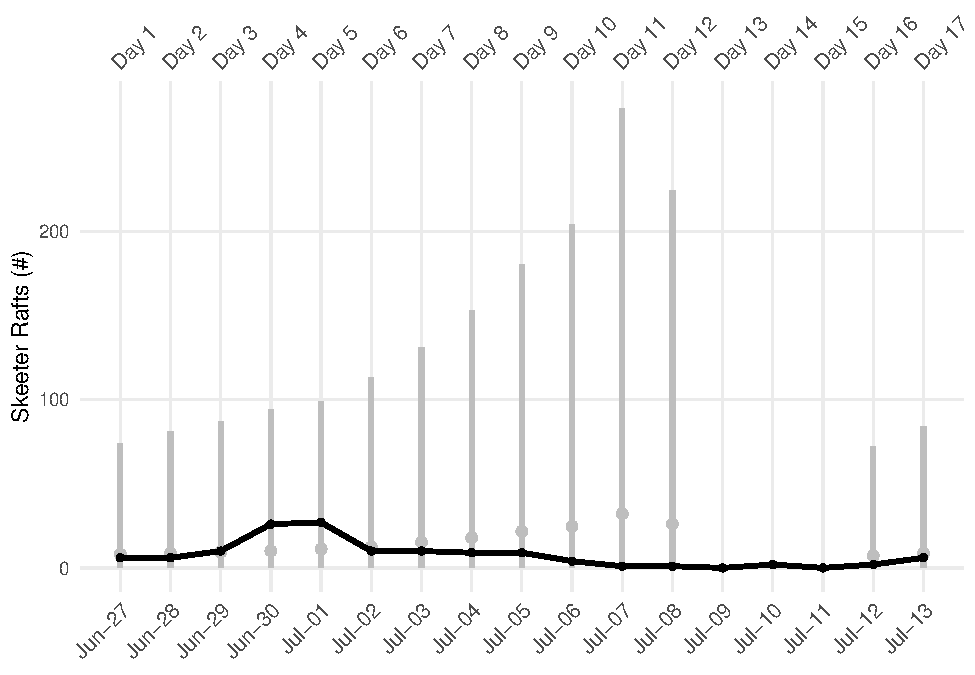
\includegraphics{skeeter-forecast-template_files/figure-latex/nb glmm plot-1.pdf}

\begin{longtable}[t]{rrrrr}
\caption{\label{tab:nb glmm accuracy}Mean predictive error of a simple Negative Binomial model}\\
\toprule
2024-06-28 & 2024-06-29 & 2024-06-30 & 2024-07-01 & MAE\\
\midrule
-6 & -15 & -43 & -28 & 23\\
\bottomrule
\end{longtable}

\subsubsection{GAMM prediction}\label{gamm-prediction}

more forecasts to come???

\end{document}
